%%%%%%%%%%%%%%%%%%%%%%%%%%%%%%%%%%%%%%%%%
% Beamer Presentation
% LaTeX Template
% Version 1.0 (10/11/12)
%
% This template has been downloaded from:
% http://www.LaTeXTemplates.com
%
% License:
% CC BY-NC-SA 3.0 (http://creativecommons.org/licenses/by-nc-sa/3.0/)
%
%%%%%%%%%%%%%%%%%%%%%%%%%%%%%%%%%%%%%%%%%

%----------------------------------------------------------------------------------------
%	PACKAGES AND THEMES
%----------------------------------------------------------------------------------------

\documentclass{beamer}

%----------------------------------------------------------------------------------------
%	IMPORTACIONES
%----------------------------------------------------------------------------------------

\usepackage{amssymb}% http://ctan.org/pkg/amssymb
\usepackage{pifont}% http://ctan.org/pkg/pifont
\newcommand{\cmark}{\ding{51}}%
\newcommand{\xmark}{\ding{55}}%

%paquete usado para silabación en español
\usepackage[spanish]{babel}
%codificación del documento
\usepackage[utf8]{inputenc}

\mode<presentation> {

% The Beamer class comes with a number of default slide themes
% which change the colors and layouts of slides. Below this is a list
% of all the themes, uncomment each in turn to see what they look like.

%\usetheme{default}
%\usetheme{AnnArbor}
%\usetheme{Antibes}
%\usetheme{Bergen}
%\usetheme{Berkeley}
\usetheme{Berlin}
%\usetheme{Boadilla}
%\usetheme{CambridgeUS}
%\usetheme{Copenhagen}
%\usetheme{Darmstadt}
%\usetheme{Dresden}
%\usetheme{Frankfurt}
%\usetheme{Goettingen}
%\usetheme{Hannover}
%\usetheme{Ilmenau}
%\usetheme{JuanLesPins}
%\usetheme{Luebeck}
%\usetheme{Madrid}
%\usetheme{Malmoe}
%\usetheme{Marburg}
%\usetheme{Montpellier}
%\usetheme{PaloAlto}
%\usetheme{Pittsburgh}
%\usetheme{Rochester}
%\usetheme{Singapore}
%\usetheme{Szeged}
%\usetheme{Warsaw}

% As well as themes, the Beamer class has a number of color themes
% for any slide theme. Uncomment each of these in turn to see how it
% changes the colors of your current slide theme.

%\usecolortheme{albatross}
%\usecolortheme{beaver}
%\usecolortheme{beetle}
%\usecolortheme{crane}
%\usecolortheme{dolphin}
%\usecolortheme{dove}
%\usecolortheme{fly}
%\usecolortheme{lily}
%\usecolortheme{orchid}
%\usecolortheme{rose}
%\usecolortheme{seagull}
%\usecolortheme{seahorse}
%\usecolortheme{whale}
%\usecolortheme{wolverine}

%\setbeamertemplate{footline} % To remove the footer line in all slides uncomment this line
%\setbeamertemplate{footline}[page number] % To replace the footer line in all slides with a simple slide count uncomment this line

%\setbeamertemplate{navigation symbols}{} % To remove the navigation symbols from the bottom of all slides uncomment this line
}

\usepackage{graphicx} % Allows including images
\usepackage{booktabs} % Allows the use of \toprule, \midrule and \bottomrule in tables

%----------------------------------------------------------------------------------------
%	TITLE PAGE
%----------------------------------------------------------------------------------------

\title[SEPA 2.0]{MÓDULOS INTEGRADOR Y MANTENEDOR DE DATOS EN SISTEMA SEPA VERSION 2.0} % The short title appears at the bottom of every slide, the full title is only on the title page

\author{Miguel Ángel Aníbal Davor Fuenzalida Pino} % Your name
\institute[UTEM] % Your institution as it will appear on the bottom of every slide, may be shorthand to save space
{
UNIVERSIDAD TECNOLÓGICA METROPOLITANA \\ % Your institution for the title page
\medskip
\textit{anibaldavor@gmail.com} % Your email address
}
\date{\today} % Date, can be changed to a custom date

\begin{document}

\begin{frame}
\titlepage % Print the title page as the first slide
\end{frame}

\begin{frame}
\frametitle{Contenidos} % Table of contents slide, comment this block out to remove it
\tableofcontents % Throughout your presentation, if you choose to use \section{} and \subsection{} commands, these will automatically be printed on this slide as an overview of your presentation
\end{frame}

%----------------------------------------------------------------------------------------
%	PRESENTATION SLIDES
%----------------------------------------------------------------------------------------

\section{Análisis}

\subsection{Resumen}

\begin{frame}
\frametitle{SEPA Anterior}
\begin{itemize}
\item Datos provenientes de DirDoc, proceso de traspaso inseguro.
\item Carece de formas alternativas de acceso.
\item Falta de roles para los usuarios.
\item No es posible reparar datos incompletos.
\end{itemize}
\end{frame}

%------------------------------------------------

\begin{frame}
\frametitle{SEPA Nuevo}
\begin{itemize}
\item Mantenedor: Versión actualizada de SEPA.
\item Integrador: Rescate de información automático.
\end{itemize}
\end{frame}

%------------------------------------------------

\begin{frame}
\frametitle{Beneficios}
\begin{itemize}
\item Información que otorga una mejor perspectiva de la realidad universitaria.
\item Mirar el desempeño académico de un estudiante.
\item Integrar componentes o funcionalidades a SEPA 2.0.
\item Extracción de data en forma segura y automática.
\end{itemize}
\end{frame}

%------------------------------------------------

\begin{frame}
\frametitle{Situación final}
\begin{itemize}
\item Ingreso por perfiles.
\item Visualización de todas las tablas que componen la base de datos.
\item Mantenedor de perfiles.
\item Web Service integrador.
\item Expansibilidad.
\end{itemize}
\end{frame}

%------------------------------------------------

\subsection{Proceso}

\begin{frame}
\frametitle{Objetivos}
\begin{block}{General}
Actualizar SEPA a una versión 2.0, creando un sistema actualizado e independiente de información estadística para la Universidad Tecnológica Metropolitana ayudando a sus procesos docentes y productivos, disponiendo de información veraz a la realidad universitaria.
\end{block}


\begin{itemize}
\item Sistema simple de mejorar.
\item Desarrollado bajo herramientas robustas.
\item Creación de un SEPA 2.0 diferente de su predecesor.
\end{itemize}
\end{frame}

%------------------------------------------------

\begin{frame}
\frametitle{Diagrama del proyecto}
\begin{figure}[!hbp]
\begin{center}
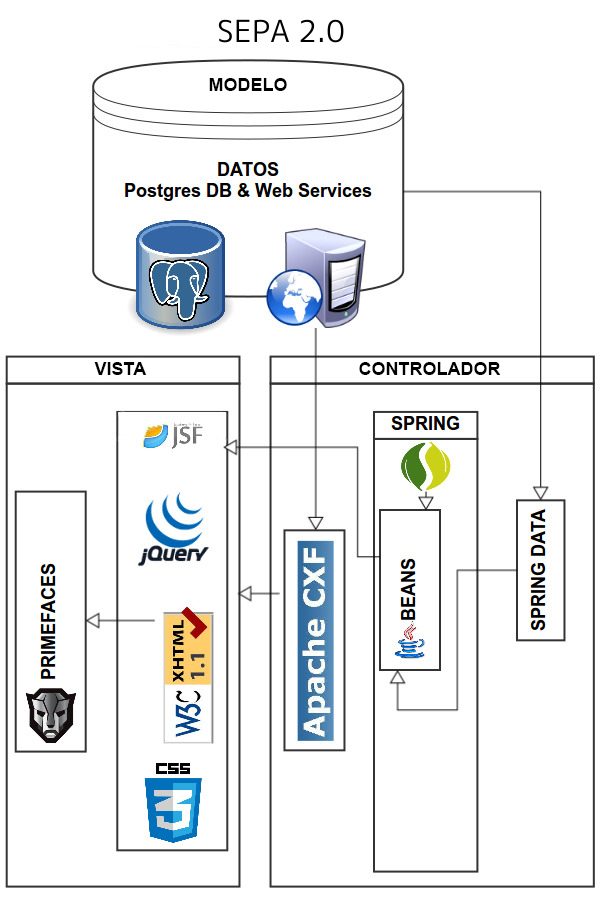
\includegraphics[scale=0.2,angle=0]{images/diagrama2.jpg}
\caption{Diagrama general del sistema}
\label{Diagrama general del sistema}
\end{center}
\end{figure}
\end{frame}

%------------------------------------------------

\begin{frame}
\frametitle{Ciclo de Vida}
\begin{figure}[!hbp]
\begin{center}
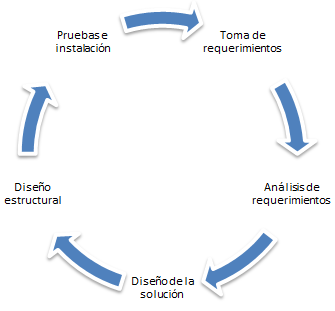
\includegraphics[scale=0.6,angle=0]{images/cicloMini.PNG}
\caption{Ciclo de vida}
\label{Organigrama de rectoria}
\end{center}
\end{figure}
\end{frame}

%------------------------------------------------

\begin{frame}
\frametitle{Estado del Arte}
\begin{block}{QS Top Universities}
Evaluación mediante ránkings enfocados a entregar información a organismos y personas relacionadas con post-grados, MBA, estudios de ingeniería y negocios.
\end{block}
\begin{block}{Ránking de Calidad de las Universidades Chilenas}
Ránking para instituciones educacionales en Chile, que utiliza ciertos criterios, como son la cantidad de investigaciones o la masa de estudiantes que entran en cada Universidad \cite{p1}.
\end{block}
\end{frame}

%------------------------------------------------

\begin{frame}
\frametitle{Análisis de las Herramientas}
\begin{table}
\begin{tabular}{l l l l l}
\toprule
				& \textbf{php} & \textbf{.net} & \textbf{Rails} & \textbf{Java}\\
\midrule
Sencillez 		& \textcolor{green}{\cmark} & \textcolor{red}{\xmark}   & \textcolor{red}{\xmark}   &\textcolor{green}{\cmark}\\
Robustez 		& \textcolor{red}{\xmark}   & \textcolor{green}{\cmark} & \textcolor{green}{\cmark} &\textcolor{green}{\cmark}\\
Seguridad 		& \textcolor{red}{\xmark}   & \textcolor{red}{\xmark}   & \textcolor{green}{\cmark} &\textcolor{green}{\cmark}\\
Portabilidad 	& \textcolor{green}{\cmark} & \textcolor{red}{\xmark}   & \textcolor{red}{\xmark}   &\textcolor{green}{\cmark}\\
Neutralidad 	& \textcolor{green}{\cmark} & \textcolor{red}{\xmark}   & \textcolor{green}{\cmark} &\textcolor{green}{\cmark}\\
Interfaz 		& \textcolor{red}{\xmark}   & \textcolor{green}{\cmark} & \textcolor{green}{\cmark} &\textcolor{green}{\cmark}\\
Expresividad 	& \textcolor{green}{\cmark} & \textcolor{red}{\xmark}   & \textcolor{green}{\cmark} &\textcolor{red}{\xmark}\\
Compilación 	& \textcolor{green}{\cmark} & \textcolor{red}{\xmark}   & \textcolor{green}{\cmark} &\textcolor{red}{\xmark}\\
Aprendizaje 	& \textcolor{green}{\cmark} & \textcolor{red}{\xmark}   & \textcolor{green}{\cmark} &\textcolor{green}{\cmark}\\
E. de control 	& \textcolor{green}{\cmark} & \textcolor{green}{\cmark} & \textcolor{green}{\cmark} &\textcolor{green}{\cmark}\\
Abstracción 	& \textcolor{green}{\cmark} & \textcolor{red}{\xmark}   & \textcolor{red}{\xmark}   &\textcolor{green}{\cmark}\\
\textbf{Total}  & 8 & 3 & 8 & 9\\
\bottomrule
\end{tabular}
\caption{Table caption}
\end{table}
\end{frame}

%------------------------------------------------

\section{Proyecto}

\subsection{Preámbulo}

%------------------------------------------------

\begin{frame}
\frametitle{Criterios de Calidad}
\begin{itemize}
\item \textbf{Mantenibilidad}: Modelo de programación simple para corregir.
\item \textbf{Flexibilidad}: Capacidad de crecimiento del código.
\item \textbf{Testeabilidad}: Test de funcionamiento.
\item \textbf{Portabilidad}: Portabilidad sobre muchos S.O. en distintas arquitecturas
\item \textbf{Integridad}: Integridad de la data que es ingresada.
\item \textbf{Rapidez}: Ejecución de servicios de forma veloz y clara.
\end{itemize}
\end{frame}

%------------------------------------------------

\begin{frame}
\frametitle{Patrones de Diseño}
\begin{itemize}
\item \textbf{MVC}: Modelo Vista Controlador
\item \textbf{SOA}: Arquitectura orientada a servicios
\item \textbf{POA}: Programación Orientada al Aspecto
\item \textbf{DAO}: Objeto de Acceso a datos
\end{itemize}
\end{frame}

\subsection{Desarrollo}

%------------------------------------------------

\begin{frame}
\frametitle{Integrador}
\begin{itemize}
\item \textbf{Poblador}: Herramienta desarrollada con el fin de buscar los datos desde DirDoc de manera segura y controlada.
\item \textbf{Periodicidad}: Característica del poblador que establece fechas, horas y minutos en donde varios servicios consultan datos.
\item \textbf{Web Service}: Framework que permite la comunicación entre 2 sistemas mediante un lenguaje de marcado expuesto por el que envia y el receptor.
\end{itemize}
\end{frame}

%------------------------------------------------

\begin{frame}
\frametitle{Operaciones}
\begin{itemize}
\item \textbf{Tarea Diaria}: Actualizar Cohortes y Estudiantes.
\item \textbf{Tarea Semanal}: Actualizar Asignaturas Cursadas.
\item \textbf{Tarea Mensual}: Actualizar Cursos, Docentes y Cargos.
\item \textbf{Tarea Trimestral}: Actualizar Asignaturas, Cupos Carreras y Titulados.
\item \textbf{Tarea Semestral}: Actualizar Establecimientos.
\item \textbf{Tarea Anual}: Actualizar Carreras, Planes de Estudio y Quintalización
\end{itemize}
\end{frame}

%------------------------------------------------

\begin{frame}
\frametitle{Tabla Comparativa (Integrador)}
\begin{table}
\begin{tabular}{l l l l}
\toprule
\textbf{SEPA} & \textbf{Hoy} & \textbf{2.0} & Característica\\
\midrule
Instalación 	& \textcolor{green}{\cmark} & \textcolor{green}{\cmark} & Servidor de aplicaciones  \\
Uso		 		& \textcolor{green}{\cmark} & \textcolor{green}{\cmark} & Uso automático \\
Monitoreo 		& \textcolor{red}{\xmark}   & \textcolor{green}{\cmark} & Genera alertas debido a fallos \\
Portabilidad 	& \textcolor{red}{\xmark}   & \textcolor{green}{\cmark} & Se puede reinstalar \\
Estabilidad 	& \textcolor{red}{\xmark}   & \textcolor{green}{\cmark} & Presenta pocos o nulos fallos \\
\bottomrule
\end{tabular}
\end{table}
\end{frame}

%------------------------------------------------

\begin{frame}
\frametitle{Mantenedor}
\begin{itemize}
\item \textbf{Sitio Web}: Es un módulo que permite a distintos usuarios desarrollar tareas como consultar y editar sobre un grupo acotado de tablas.
\item \textbf{Perfiles}: Característica que incide en el ámbito de visualización de cada usuario de SEPA.
\item \textbf{Ingreso}: Herramienta que verificación de Usuarios contrastados con su Perfil.
\end{itemize}
\end{frame}

%------------------------------------------------

\begin{frame}
\frametitle{Mantenedores (Modelo)}
\begin{itemize}
\item \textbf{Inicio}: Mensaje de bienvenida y punto de partida.
\item \textbf{Acceso}: Acceso, Auditoría, Rol y Usuario.
\item \textbf{Geografía}: País, Región, Provincia y Comuna.
\item \textbf{Utem}: Facultad, Departamento, Escuela, Contrato, Docente, Jerarquía, Jornada, Carrera, Asignatura Malla, Cupo Carrera, Malla, Plan de Estudio y Requisito de Asignatura.
\item \textbf{Curso}: Asignatura, Asignatura Cursada, Curso, Estado de Asignatura y Régimen.
\item \textbf{Estudiante}: Establecimiento, Grupo Dependencia, Rama, Régimen Educacional, Tipo Establecimiento, Cohorte, Egresado, Estado Alumno, Estudiante, Histórico Alumno, Tipo de Ingreso y Titulado.
\item \textbf{Contacto}: Contacto y Preguntas Frecuentes.
\item \textbf{Sesión}: Logout para poder salir del sistema cerrando sesión.
\end{itemize}
\end{frame}

%------------------------------------------------

\begin{frame}
\frametitle{Tabla Comparativa (Mantenedor)}
\begin{table}
\begin{tabular}{l l l l}
\toprule
\textbf{SEPA} & \textbf{Hoy} & \textbf{2.0} & Característica\\
\midrule
Instalación 	& \textcolor{green}{\cmark} & \textcolor{green}{\cmark} & Servidor de aplicaciones  \\
Uso		 		& \textcolor{green}{\cmark} & \textcolor{green}{\cmark} & Uso intuitivo \\
Monitoreo 		& \textcolor{green}{\cmark} & \textcolor{green}{\cmark} & Genera alertas debido a fallos \\
Portabilidad 	& \textcolor{red}{\xmark}   & \textcolor{green}{\cmark} & Se puede reinstalar \\
Estabilidad 	& \textcolor{red}{\xmark}   & \textcolor{green}{\cmark} & Presenta pocos o nulos fallos \\
\bottomrule
\end{tabular}
\end{table}
\end{frame}

%------------------------------------------------

\section{Resultados} 

\subsection{Evaluación}

%------------------------------------------------

\begin{frame}
\frametitle{Estimación de Costos}
\begin{block}{COCOMO (Modelo Constructivo de Costos)}
Es un proceso que gana fuerza con proyectos que van creciendo a medida que se van desarrollando, por lo cual esta orientado a la estimación de lo que es el producto final. Este proceso particularmente mide el tamaño del proyecto, pero no su funcionalidad.
\end{block}
\begin{block}{Punto Función}
Evaluación del impacto de cada componente realizada. Esta enfocado a los distintos tipos de desarrollo que uno debe hacer en un proyecto, utilizando una categorización de tal manera que se tiene en cuenta el impacto en conjunto de todas estas piezas.
\end{block}
\end{frame}

%------------------------------------------------

\begin{frame}
\frametitle{Conteo de puntos}
\begin{itemize}
\item \textbf{Ficheros Internos Lógicos}: Cantidad de información de los datos internos, contenida en bases de datos y ficheros de configuración.
\item \textbf{Ficheros Externos de Interfaz}: Datos externos que son administrados por la aplicación DirDoc.
\item \textbf{Entrada Externa}: Servicios web provenientes de otros sistemas.
\item \textbf{Salida Externa}: Muestra la totalidad de los datos internos en su parte visual.
\item \textbf{Consulta Externa}: Mantenedores de todos sus datos en base de datos, para poder ser modificables por los usuarios.
\end{itemize}
\end{frame}

%------------------------------------------------

\begin{frame}
\frametitle{Tabla de valores ponderados}
\begin{table}
\begin{tabular}{l c l c c}
\toprule
\textbf{Carac.} & \textbf{Pond.} & \textbf{Valor} & \textbf{Deter.} & \textbf{Total}\\
\midrule
FIL & 49 & medio & 8 & 8x4 \\
FEI	& 43 & medio & 3 &  3x5\\
EE 	& 16 & alto  & 6 &  6x10\\
SE 	& 43 & alto  & 8 &  8x25\\
CE	& 43 & alto  & 8 &  8x15\\
\textbf{Total} &&&   &  427\\
\bottomrule
\end{tabular}
\end{table}
\end{frame}

%------------------------------------------------

\begin{frame}
\frametitle{Características Generales del Sistema (puntos)}
\begin{columns}[c] % The "c" option specifies centered vertical alignment while the "t" option is used for top vertical alignment

\column{.45\textwidth} % Left column and width
\begin{itemize}
\item Datos Comunicados [4]
\item Proceso Distribuido [4]
\item Rendimiento [4]
\item Explotación [1]
\item Transacciones [2]
\item Entradas ON-LINE [5]
\item Eficiencia [3]
\end{itemize}

\column{.5\textwidth} % Right column and width
\begin{itemize}
\item Actualizaciones ON-LINE [4]
\item Lógica Interna Compleja [5]
\item Reusabilidad del Código [5]
\item Conversión e Instalación [0]
\item Facilidad de Operación [5]
\item Instalaciones Múltiples [3]
\item Facilidad de Cambios [3]
\end{itemize}

\end{columns}
\end{frame}

%------------------------------------------------

\begin{frame}
\frametitle{Valor Final}
\begin{theorem}[Calculo Puntos de Función Ajustados]
$PFA = PFSA x (0,65 + (0,01 x FCT) = 427 x (0,65 + (0,01 x 48) = 452,51$
\end{theorem}
\begin{theorem}[Calculo Horas Hombre]
$452,51PF x 4(HH/PF) = 452,51 x (4)HH = 1810,04HH$
\end{theorem}
\begin{theorem}[Valor Final]
$1810,04HH x 0,9(UF/HH) = 1629UF = 40,931,435Pesos$
\end{theorem}
\end{frame}

%------------------------------------------------

\subsection{Conclusión}

%------------------------------------------------

\begin{frame}
\frametitle{Garantías de calidad}
\begin{itemize}
\item \textbf{Postgre SQL}: Sistema gestor de bases de datos altamente estable \cite{p2}.
\item \textbf{Spring Data}: Framework JPA para el control de los datos desde múltiples fuentes \cite{p3}.
\item \textbf{Web Service CXF}: Sistema de comunicación entre 2 servicios mediante un protocolo común \cite{p4}.
\item \textbf{Primefaces JSF}: Motor para generar interfaces de usuario avanzadas y simples \cite{p5}.
\item \textbf{MVC}: Modelo de desarrollo computacional para el manejo de grandes proyectos.
\end{itemize}
\end{frame}

%------------------------------------------------

\begin{frame}
\frametitle{Conclusión Final}
\begin{block}{}
Importante oportunidad de mejoras, tales como: mantenibilidad de la data, aunque esta contenga errores, ya que es posible editar aspectos mínimos dentro de todas las tablas, conectividad con servicios web, manejado por parámetros SOAP.
\end{block}
\end{frame}

%------------------------------------------------

\begin{frame}
\frametitle{Trabajo Futuro}
\begin{block}{}
Motor de minería de datos que revele información que hasta ahora no se ha obtenido dentro de los marcos de este proyecto, por ejemplo, una herramienta que obtenga formulaciones o métodos de aproximación para datos del futuro.
\end{block}
\begin{block}{}
Inteligencia de Negocio que junto con la idea anterior sea capaz de producir nuevos indicadores enfocados a la mejora o a la conducción, con intervención humana, de los valores generalizados en las tablas que maneja SEPA.
\end{block}
\end{frame}

%------------------------------------------------

\begin{frame}
\frametitle{References}
\footnotesize{
\begin{thebibliography}{99} % Beamer does not support BibTeX so references must be inserted manually as below
\bibitem[America Economia, 2010]{p1} America Economia Ránking (2010)
\newblock El Ránking de Calidad de las Universidades Chilenas
\end{thebibliography}

\begin{thebibliography}{99} % Beamer does not support BibTeX so references must be inserted manually as below
\bibitem[Douglas, 2003]{p2} Susan Douglas Korry Douglas (2003)
\newblock PostgreSQL
\newblock \emph{Sams Publishing}.
\end{thebibliography}

\begin{thebibliography}{99} % Beamer does not support BibTeX so references must be inserted manually as below
\bibitem[Hemrajani, 2006]{p3} Anil Hemrajani (2006)
\newblock Agile Java Development with Spring, Hibernate and Eclipse.
\newblock \emph{Sams Publishing}.
\end{thebibliography}

\begin{thebibliography}{99} % Beamer does not support BibTeX so references must be inserted manually as below
\bibitem[Kalin, 2013]{p4} Martin Kalin (2013)
\newblock Java Web Services
\newblock \emph{Reilly Media}.
\end{thebibliography}

\begin{thebibliography}{99} % Beamer does not support BibTeX so references must be inserted manually as below
\bibitem[Varaksin, 2006]{p5} Oleg Varaksin (2006)
\newblock Beginning JSP, JSF and Tomcat
\end{thebibliography}
}
\end{frame}

%------------------------------------------------

\begin{frame}
\Huge{\centerline{Demo SEPA 2.0}}
\end{frame}

%----------------------------------------------------------------------------------------

\end{document} 